%%%%%%%%%%%%%%%%%%%%%%% file template.tex %%%%%%%%%%%%%%%%%%%%%%%%%
%
% This is a general template file for the LaTeX package SVJour3
% for Springer journals.          Springer Heidelberg 2010/09/16
%
% Copy it to a new file with a new name and use it as the basis
% for your article. Delete % signs as needed.
%
% This template includes a few options for different layouts and
% content for various journals. Please consult a previous issue of
% your journal as needed.
%
%%%%%%%%%%%%%%%%%%%%%%%%%%%%%%%%%%%%%%%%%%%%%%%%%%%%%%%%%%%%%%%%%%%
%
% First comes an example EPS file -- just ignore it and
% proceed on the \documentclass line
% your LaTeX will extract the file if required
\begin{filecontents*}{example.eps}
%!PS-Adobe-3.0 EPSF-3.0
%%BoundingBox: 19 19 221 221
%%CreationDate: Mon Sep 29 1997
%%Creator: programmed by hand (JK)
%%EndComments

gsave
newpath
  20 20 moveto
  20 220 lineto
  220 220 lineto
  220 20 lineto
closepath
2 setlinewidth
gsave
  .4 setgray fill
grestore
stroke
grestore
\end{filecontents*}
%
\RequirePackage{fix-cm}
%
%\documentclass{svjour3}                     % onecolumn (standard format)
%\documentclass[smallcondensed]{svjour3}     % onecolumn (ditto)
%\documentclass[smallextended]{svjour3}       % onecolumn (second format)
\documentclass[twocolumn, draft]{svjour3}          % twocolumn
%
\smartqed  % flush right qed marks, e.g. at end of proof
%



% \usepackage{mathptmx}      % use Times fonts if available on your TeX system
%
% insert here the call for the packages your document requires
%\usepackage{latexsym}
\usepackage{graphicx}
\usepackage{blindtext}
\usepackage[utf8]{inputenc}
\usepackage{booktabs}
\usepackage{tikz}
    \usetikzlibrary{arrows, matrix, calc, shapes.geometric, shapes.misc,positioning}
\usepackage{adjustbox}
\usepackage{subfig}
\usepackage{xcolor}

\let\proof\relax
\let\endproof\relax

\usepackage{amsfonts, amsmath, amsthm, amssymb}
\usepackage[utf8]{inputenc}
\usepackage[numbers, sort, compress]{natbib}
\usepackage{pifont}% http://ctan.org/pkg/pifont
	\newcommand{\cmark}{\ding{51}}%
  \newcommand{\xmark}{\ding{53}}%


% please place your own definitions here and don't use \def but
% \newcommand{}{}
%
% Insert the name of "your journal" with
% \journalname{myjournal}
%
\begin{document}

\title{Semantic Segmentation for Skin Melanoma Detection%\thanks{Grants or other notes
%about the article that should go on the front page should be
%placed here. General acknowledgments should be placed at the end of the article.}
}
\subtitle{A convolutional neural network implementation.}

%\titlerunning{Semantic Segmentation}        % if too long for running head

\author{Mario Alberto Flores Hernández}

%\authorrunning{Short form of author list} % if too long for running head

\date{Received: date / Accepted: date}
% The correct dates will be entered by the editor


\maketitle

\begin{abstract}
  The approach described in this paper for the detection of the skin cancer melanoma is known as semantic segmentation. The semantic segmentation is a computer vision task where the different regions of an image are classified according to a specific category. The method used for the implementation of a semantic segmentation software was using the convolutional neural network, specifically a feature pyramid network architecture (\texttt{FPN}), to train a model which performs the task. With the convolutional neural networks is possible to train models that replicate the necessary transformations to obtain a targeted output, the only requirement is a rich enough database of samples of the input data and the target or the expected output in relation with that input, which in this case was a segmentation mask of the dermoscopic image.

\keywords{Neural Network \and Convolution \and Semantic Segmentation \and Classification}
% \PACS{PACS code1 \and PACS code2 \and more}
% \subclass{MSC code1 \and MSC code2 \and more}
\end{abstract}

\section{Introduction}
Skin is considered one of the largest organs in the human body, its function is to protect the internal organs and structures from the harsh environmental conditions such as temperature, radiation and bacteria. The skin also functions as a large sensorial interface that let us feel the environment conditions such as the temperature in the ambience and feel the texture of the objects.
The skin cancer known as melanoma is one of the deadliest types of cancer if not detected in its early stages, because of the quick spread to other organs caused by the metastasis effect. One way to reduce its mortality rate is by using automatic detection with computer vision technologies, such as the deep learning technology. With deep learning is possible to train models that recognize the presence of the melanoma tissue using a configuration of parameters fine-tuned during a process known as \emph{training} which compares the input of the model and the known output to that input, and then update the parameters to get the computed output closer to the known output.


\section{Background}
In this section are introduced the basic concepts an theories required to understand the following proposals. Starting with some basic background aspects about the melanoma cancer, then continuing with the loss functions and the optimizer functions.

\definecolor{red_matrix}{rgb}{0.6, 0, 0}
\definecolor{green_matrix}{rgb}{0, 0.8, 0}
\definecolor{blue_matrix}{rgb}{0, 0.25, 1}

\begin{figure*}[htp]
  \centering
  \subfloat[Grayscale.]{
      \label{mtr_1}
      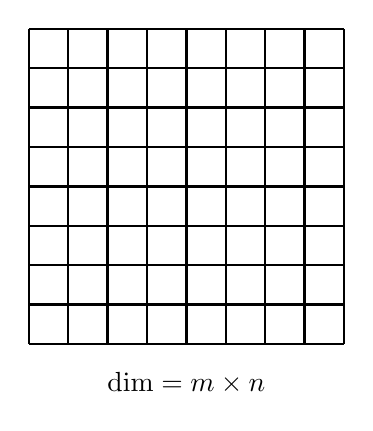
\begin{tikzpicture}
          \draw[step=5mm, black, line width=0.30mm] (-2,-2) grid (2,2);
          \node at (0,-2.5) {$\text{dim} = m \times n$};
      \end{tikzpicture}
  }
  \qquad
  \subfloat[Color.]{
      \label{mtr_2} 
      \begin{tikzpicture}
          \draw[step=5mm, red_matrix, line width=0.30mm] (-2.5,-2.5) grid (1.5,1.5);
          \draw[step=5mm, green_matrix, line width=0.30mm] (-2,-2) grid (2,2);
          \draw[step=5mm, blue, line width=0.30mm] (-1.5,-1.5) grid (2.5,2.5);
          \node at (0, -3) {$\text{dim} = m \times n \times k$};
      \end{tikzpicture}
  }
  \caption{Dimensional comparison between images.}
\end{figure*}



\section{Related Work}
In this section the related works were summarized to make a comparison between different methods to approach the melanoma detection problem and same approaches for the solution of different problems and get an idea of the opportunity areas and the advantages and disadvantages of the proposed solution.

\begin{table}[h!]
  \begin{center}
  \scalebox{0.5}{
      \begin{tabular}[t]{|l|l|l|l|l|l|l|l|}
          \hline
          \bf{Work} & \bf{Model} & \bf{\rotatebox{90}{Classification}} & \bf{\rotatebox{90}{Segmentation}} & \bf{\rotatebox{90}{Supervised}} & \bf{\rotatebox{90}{Pre-train\phantom{m}}} & \bf{\rotatebox{90}{Evaluation}} & \bf{Output}\\
          \hline
          \citet{DBLP:journals/corr/BadrinarayananK15} & \texttt{SegNet} & \cmark & \cmark & \cmark & \cmark & \cmark & mapa de etiquetas\\
          \citet{DBLP:journals/corr/RonnebergerFB15} & \texttt{U-net} & \cmark & \cmark & \cmark & \xmark & \cmark & mapa de etiquetas\\
          \citet{DBLP:journals/corr/ChenPK0Y16} & \texttt{DeepLab} & \cmark & \cmark & \cmark & \xmark & \cmark & mapa de etiquetas\\   
          \citet{DBLP:journals/corr/TeichmannWZCU16} & \texttt{MultiNet} & \cmark & \cmark & \cmark & \xmark & \cmark & mapa de etiquetas\\   
          \citet{KRONER2020261} & \texttt{VGG16} & \cmark & \cmark & \cmark & \cmark & \cmark & mapa de calor\\ 
          \citet{KADAMPUR2020100282} & \texttt{CNN} & \cmark & \xmark & \cmark & \xmark & \cmark & mapa de etiquetas\\    
          \citet{zhou2019emerging} & \texttt{ML / SVM} & \cmark & \xmark & \cmark & \xmark & \cmark & etiqueta\\    
          \citet{DBLP:journals/corr/LucCCV16} & \texttt{CNN/GAN} & \cmark & \cmark & \cmark & \cmark & \cmark & mapa de etiquetas\\         
          \citet{JAIN2015735} & \texttt{A.B.C.D} & \xmark & \cmark & \xmark & \xmark & \xmark & etiqueta\\
          \hline
          Propuesta de tesis & \texttt{FPN} & \cmark & \cmark & \cmark & \cmark & \cmark & mapa de etiquetas\\
          \hline   
      \end{tabular}
      }
  \end{center}
  \label{Tab:comp_1}
\end{table}

\section{Proposed Solution}
The approach proposed in this paper for the automated detection of the skin melanoma is the training of a model using a \texttt{FPN} convolutional neural network architecture, which output would be the probabilistic map of the regions inside of the dermoscopic input image. The language selected for the implementation of said neural network architecture was \texttt{Python}, because is a powerful, dynamic and quick to deploy language which also contains the \texttt{Torch} library which is the core tool of the implementation.

\section{Experiments}
The methods used to evaluate the performance of the training process and also gauge the probabilistic map predictions are described in this section. Also the analysis of the threshold is included here.

\begin{center}
  \begin{equation}\label{eq:dice_loss}
      \text{CD} = \frac{2|A \cap B |}{|A| + |B|}
  \end{equation}        
\end{center}

\begin{equation}\label{eq:jacc}
  \text{CJ} = \frac{|A \cap B|}{| A \cup B |} = \frac{|A \cap B|}{|A| + |B| - |A \cap B|} \text{,}
\end{equation}

\begin{table}[h]
  \centering
  \begin{tabular}{c c c}
    \toprule
    \textbf{Epoch} & \textbf{DL} & \textbf{IoU} \\
    \midrule
    1 & 0.2968 & 0.5616 \\
    2 & 0.2972 & 0.5546 \\
    3 & 0.2690 & 0.5879 \\
    4 & 0.2960 & 0.6389 \\
    5 & 0.2371 & 0.8415 \\
    6 & 0.0929 & 0.8626 \\
    7 & 0.0792 & 0.8626 \\
    8 & 0.0692 & 0.8798 \\
    9 & 0.0556 & 0.9017 \\
    10 & 0.0542 & 0.9039 \\
    \bottomrule
    
  \end{tabular}
\end{table}
\section{Conclusion}

%\begin{acknowledgements}
%If you'd like to thank anyone, place your comments here
%and remove the percent signs.
%\end{acknowledgements}


% Authors must disclose all relationships or interests that 
% could have direct or potential influence or impart bias on 
% the work: 
%
% \section*{Conflict of interest}
%
% The authors declare that they have no conflict of interest.
\section{References}

% BibTeX users please use one of
%\bibliographystyle{spbasic}      % basic style, author-year citations
%\bibliographystyle{spmpsci}      % mathematics and physical sciences
%\bibliographystyle{spphys}       % APS-like style for physics
\bibliographystyle{mighelnat}    % FIME - Custom Style.

\footnotesize
\bibliography{MiBiblio}   % name your BibTeX data base

% Non-BibTeX users please use
%\begin{thebibliography}{}
%
% and use \bibitem to create references. Consult the Instructions
% for authors for reference list style.
%
%\bibitem{RefJ}
% Format for Journal Reference
%Author, Article title, Journal, Volume, page numbers (year)
% Format for books
%\bibitem{RefB}
%Author, Book title, page numbers. Publisher, place (year)
% etc
%\end{thebibliography}

\end{document}
% end of file template.tex

